\cotefile{29}
\scanpage{102}
\mspage{101}
\margin{\figure{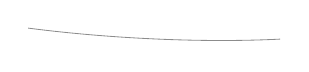
\begin{tikzpicture}\draw[black!45,line width=.3pt] (0,0) .. controls (1,-.13) and (2.2,-.19) .. (3.2,-.14);\end{tikzpicture}}}

Examinons maintenant le cas où l'un des cycles $\underline{a}$ ou $\underline{b}$ (par exemple $\underline{b}$) appartient au noyau d'Albanese $Z_{\handwritten{\ell}}(A)$ ; par linéarité, on se ramène au cas où $\underline{b}$ est de la forme $\underline{c}_u-\underline{c}$, avec $\underline{c}\handwritten{\in}Z^{s}_{\unsure{o|0}}(A)_{\bar{\underline{k}}}$, et $u\handwritten{\in}{}^{s}A_{\bar{\underline{k}}}$. D'après l'invariance du symbole $j_{\handwritten{o}}$ par la translation $\handwritten{\tau_u}$, les deux membres de (3) sont respectivement égaux à $j_{\handwritten{o}}(Y_{\underline{a}},\underline{c})$ et à $j_{\handwritten{o}}(Y^{-}_{\underline{c}},\underline{a})$\inserted{\handwritten{, en posant $Y=X_u-X$.}} Puisqu'on a $X\handwritten{\in}D_a(A)$, on a $Y\handwritten{\sim}0$, et on est ramené au cas déjà traité.

Supposons maintenant $X$, $\underline{a}$ et $\underline{b}$ quelconques. On peut, en modifiant $\underline{b}$ par l'addition d'un élément de $Z^{\handwritten{s}}_{\handwritten{\ell}}(A)_{\handwritten{\bar{\underline{k}}}}$, se ramener au cas où le cycle $\underline{a}^{-}\handwritten{\otimes}\underline{b}$ est étranger à $X$. Les symboles $X_{\underline{a}}(\underline{b})$ et $X^{-}_{\underline{b}}(\underline{a})$ sont alors définis, et on a
\[
X_{\underline{a}}(\underline{b})=X^{-}_{\underline{b}}(\underline{a}),\quad\text{d'où}\quad v(X_{\underline{a}}(\underline{b}))=v(X^{-}_{\underline{b}}(\underline{a})).
\]

D'autre part, soit $a$ (resp. $b$) l'un quelconque des composants de $\underline{a}$ (resp. $\underline{b}$). Alors les symboles $i(X_a,b)$ et $i(X^{-}_b,a)$ sont définis ; l'application $\handwritten{\zeta}:A\handwritten{\longrightarrow}A$ définie par $\handwritten{\zeta}(x)=a+b-x$ étant \uline{p}-isomorphique en $b^{\handwritten{\unsure{\circ|o|0}}}$, de valeur $a^{\handwritten{\circ}}$, on a, d'après la propriété d'invariance du symbole $i$,
\[
i(X_a,b)=i(X^{-}_b,a).
\]

Il en résulte, par linéarité,
\[
i(X_{\underline{a}},\underline{b})=i(X^{-}_{\underline{b}},\underline{a}).
\]
\margin{\figure{\begin{tikzpicture}[x=1cm,y=1cm]
\fill[black!35] (0,0) .. controls (-.004,-.04) and (.006,-.08) .. (.018,-.11) .. controls (.023,-.14) and (.020,-.17) .. (.026,-.20) .. controls (.040,-.24) and (.045,-.28) .. (.037,-.30) .. controls (.018,-.31) and (.009,-.27) .. (.013,-.24) .. controls (.020,-.21) and (.022,-.20) .. (.012,-.18) .. controls (.005,-.15) and (.011,-.13) .. (.008,-.10) .. controls (-.003,-.06) and (-.006,-.02) .. (0,0);
\fill[black] (.019,-.12) .. controls (.030,-.14) and (.022,-.17) .. (.026,-.18) .. controls (.008,-.17) and (.008,-.15) .. (.019,-.12);
\fill[black] (.024,-.22) .. controls (.034,-.24) and (.044,-.28) .. (.037,-.30) .. controls (.019,-.31) and (.011,-.28) .. (.013,-.25) .. controls (.014,-.23) and (.019,-.22) .. (.024,-.22);
\end{tikzpicture}}}

Compte tenu des formules (2) précédentes, on en déduit (3).

Notons enfin \unsure{.}que $j_{\handwritten{o}}(X,\underline{a})$ s'annule lorsque tous les composants de $A$ appartiennent au groupe ${}^{s}A_{\bar{\underline{k}},\handwritten{o}}$. En effet, soit $f$ une fonction sur $V$, définie sur $\underline{k}$, telle que

% archive sheet number: 101
